\section{Documentazione API}

In questa sezione vengono presentate le API sviluppate nel corso della terza iterazione. Come nell'iterazione precedente,
le APIs sono visualizzabili nella collezione di postman esportata. In questa iterazione, le aggiunte principali sono state relative agli use cases
UC13,UC14 e all'implementazione dell'algoritmo. Infatti, come detto in precedenza, l'integrazione nel sistema ha comportato l'aggiunta di 
due funzionalità.

\begin{itemize}
    \item API per la visualizzazione dei profili (utente/organizzatore)
    \item API per ottenere il livello di ogni utente
    \item API per chiudere le iscrizioni ad un evento e selezionare i partecipanti
    \item API per ottenere tutte le prenotazioni confermate di un partecipante
\end{itemize}

\begin{figure}[h!]
    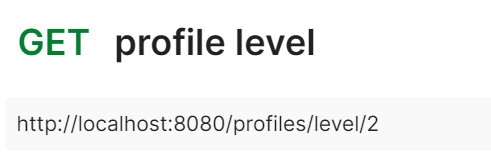
\includegraphics[width=7cm]{Iterazione 3/images/level.png}\\
    \caption{Profile level}
\end{figure}


\begin{figure}[h!]
    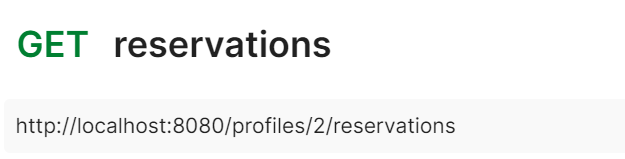
\includegraphics[width=7cm]{Iterazione 3/images/reservations.png}\\
    \caption{Ottenere tutte le prenotazioni confermate di un utente}
\end{figure}

\begin{figure}[h!]
    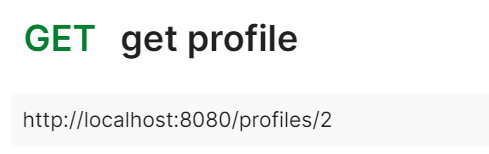
\includegraphics[width=7cm]{Iterazione 3/images/profile.png}\\
    \caption{Profilo utente}
\end{figure}

\begin{figure}[h!]
    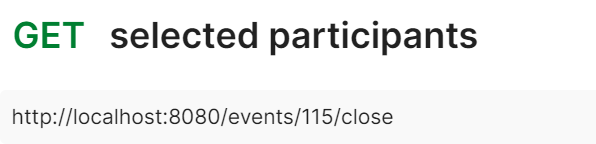
\includegraphics[width=7cm]{Iterazione 3/images/selected participants.png}\\
    \caption{Selezione partecipanti}
\end{figure}

